\chapter{Data Manipulation and Its Representation}

In this chapter a closer look two a couple more of modules is given. These modules will result to be very useful in managing financial data and to report result of our analysis.

\section{Getting Data}\label{getting-data}

The first step of any analysis is usually the one that involves selection and manipulation of data we want to process. Data sources can be various (e.g. website, figures, twitter messages, CSV or Excel files\ldots{}) and partially reflect its nature which can range from \emph{unstructured} data (without any inherent structure, e.g.~social media data) to completely \emph{structured} data (where the data model is defined and usually there is no error associated, e.g.~stock trading data).

Our primary goal, before start processing data, is to collect and store the information in a suitable data structure. \texttt{Python} provides a very useful module, called \texttt{pandas}, which allows to collect and save data in \emph{dataframe} objects that can be later on manipulated for analysis purposes.

Looking at \texttt{pandas} manual dataframe are defined as multi-dimensional, size-mutable, potentially heterogeneous, tabular data structure with labeled axes (rows and columns), in much simpler words it is a table whose structure can be modified.
It presents data in a way that is suitable for data analysis, contains multiple methods for convenient data filtering and in addition has a lot of utilities to load and save data pretty easily.

Dataframes can be created by:
\begin{itemize}
\item importing data from file;
\item creating by hand data and then filling the dataframe.
\end{itemize}


\begin{tcolorbox}[breakable, size=fbox, boxrule=1pt, pad at break*=1mm,colback=cellbackground, colframe=cellborder]
\begin{Verbatim}[commandchars=\\\{\}]
\PY{k+kn}{import} \PY{n+nn}{pandas} \PY{k}{as} \PY{n+nn}{pd}

\PY{c+c1}{\PYZsh{} reading from file}
\PY{n}{df1} \PY{o}{=} \PY{n}{pd}\PY{o}{.}\PY{n}{read\PYZus{}excel}\PY{p}{(}\PY{l+s+s1}{\PYZsq{}}\PY{l+s+s1}{sample.xlsx}\PY{l+s+s1}{\PYZsq{}}\PY{p}{)} \PY{c+c1}{\PYZsh{} Excel file}
\PY{n}{df2} \PY{o}{=} \PY{n}{pd}\PY{o}{.}\PY{n}{read\PYZus{}csv}\PY{p}{(}\PY{l+s+s1}{\PYZsq{}}\PY{l+s+s1}{sample.csv}\PY{l+s+s1}{\PYZsq{}}\PY{p}{)} \PY{c+c1}{\PYZsh{} Comma Separated file}

\PY{n}{df1}\PY{o}{.}\PY{n}{head}\PY{p}{(}\PY{l+m+mi}{11}\PY{p}{)} \PY{c+c1}{\PYZsh{} show just few rows at the beginning}

         Date       Price      Volume
0  2000-07-30  100.000000  191.811275
1  2000-07-31  129.216267  190.897541
2  2000-08-01  147.605516  197.476379
3  2000-08-02  107.282251  199.660061
4  2000-08-03  106.036826  200.840459
5  2000-08-04  118.872757  197.130212
6  2000-08-05  101.904544  204.552521
7  2000-08-06  106.392901  198.160030
8  2000-08-06  106.392901  191.125969
9  2000-08-06  106.392901  196.719061
10 2000-08-06  106.392901  196.759837
\end{Verbatim}
\end{tcolorbox}

\begin{tcolorbox}[breakable, size=fbox, boxrule=1pt, pad at break*=1mm,colback=cellbackground, colframe=cellborder]
\begin{Verbatim}[commandchars=\\\{\}]
\PY{c+c1}{\PYZsh{} creating some data in a dictionary}
\PY{n}{d} \PY{o}{=} \PY{p}{\PYZob{}}\PY{l+s+s2}{\PYZdq{}}\PY{l+s+s2}{Nome}\PY{l+s+s2}{\PYZdq{}}\PY{p}{:}\PY{p}{[}\PY{l+s+s2}{\PYZdq{}}\PY{l+s+s2}{Elisa}\PY{l+s+s2}{\PYZdq{}}\PY{p}{,} \PY{l+s+s2}{\PYZdq{}}\PY{l+s+s2}{Roberto}\PY{l+s+s2}{\PYZdq{}}\PY{p}{,} \PY{l+s+s2}{\PYZdq{}}\PY{l+s+s2}{Ciccio}\PY{l+s+s2}{\PYZdq{}}\PY{p}{,} \PY{l+s+s2}{\PYZdq{}}\PY{l+s+s2}{Topolino}\PY{l+s+s2}{\PYZdq{}}\PY{p}{,} \PY{l+s+s2}{\PYZdq{}}\PY{l+s+s2}{Gigi}\PY{l+s+s2}{\PYZdq{}}\PY{p}{]}\PY{p}{,}
     \PY{l+s+s2}{\PYZdq{}}\PY{l+s+s2}{Età}\PY{l+s+s2}{\PYZdq{}}\PY{p}{:}\PY{p}{[}\PY{l+m+mi}{1}\PY{p}{,} \PY{l+m+mi}{27}\PY{p}{,} \PY{l+m+mi}{25}\PY{p}{,} \PY{l+m+mi}{24}\PY{p}{,} \PY{l+m+mi}{31}\PY{p}{]}\PY{p}{,}
     \PY{l+s+s2}{\PYZdq{}}\PY{l+s+s2}{Punteggio}\PY{l+s+s2}{\PYZdq{}}\PY{p}{:}\PY{p}{[}\PY{l+m+mi}{100}\PY{p}{,} \PY{l+m+mi}{120}\PY{p}{,} \PY{l+m+mi}{95}\PY{p}{,} \PY{l+m+mi}{1300}\PY{p}{,} \PY{l+m+mi}{101}\PY{p}{]}\PY{p}{\PYZcb{}}

\PY{c+c1}{\PYZsh{} filling the dataframe}
\PY{n}{df} \PY{o}{=} \PY{n}{pd}\PY{o}{.}\PY{n}{DataFrame}\PY{p}{(}\PY{n}{d}\PY{p}{)}
\PY{n}{df}\PY{o}{.}\PY{n}{head}\PY{p}{(}\PY{p}{)}

       Nome  Età  Punteggio
0     Elisa    1        100
1   Roberto   27        120
2    Ciccio   25         95
3  Topolino   24       1300
4      Gigi   31        101
\end{Verbatim}
\end{tcolorbox}

Of course with \texttt{pandas} it is possible to perform a large number of operations on a dataframe. For example it is possible to add a column as a result of an operation on other columns. Looking back at the \texttt{df1} dataframe it is possible to add a column with the daily variation of the price.

\begin{tcolorbox}[breakable, size=fbox, boxrule=1pt, pad at break*=1mm,colback=cellbackground, colframe=cellborder]
\begin{Verbatim}[commandchars=\\\{\}]
\PY{k+kn}{import} \PY{n+nn}{numpy} \PY{k}{as} \PY{n+nn}{np}

\PY{c+c1}{\PYZsh{} first let\PYZsq{}s add an empty column}
\PY{n}{df1}\PY{p}{[}\PY{l+s+s1}{\PYZsq{}}\PY{l+s+s1}{Variation}\PY{l+s+s1}{\PYZsq{}}\PY{p}{]} \PY{o}{=} \PY{n}{np}\PY{o}{.}\PY{n}{nan} \PY{c+c1}{\PYZsh{} nan stands for not a number}

\PY{c+c1}{\PYZsh{} loop on the Price column, compute the variation and fill the column}
\PY{c+c1}{\PYZsh{} len returns the number of rows of a dataframe}
\PY{k}{for} \PY{n}{i} \PY{o+ow}{in} \PY{n+nb}{range}\PY{p}{(}\PY{l+m+mi}{1}\PY{p}{,} \PY{n+nb}{len}\PY{p}{(}\PY{n}{df1}\PY{p}{)}\PY{p}{)}\PY{p}{:}
    \PY{c+c1}{\PYZsh{} select the ith row and fill \PYZdq{}Variation\PYZdq{}}
    \PY{c+c1}{\PYZsh{} loc takes as inputs row and colum\PYZhy{}name}
    \PY{n}{df1}\PY{o}{.}\PY{n}{loc}\PY{p}{[}\PY{n}{i}\PY{p}{,} \PY{l+s+s2}{\PYZdq{}}\PY{l+s+s2}{Variation}\PY{l+s+s2}{\PYZdq{}}\PY{p}{]} \PY{o}{=} \PY{p}{(}\PY{n}{df1}\PY{o}{.}\PY{n}{loc}\PY{p}{[}\PY{n}{i}\PY{p}{,} \PY{l+s+s2}{\PYZdq{}}\PY{l+s+s2}{Price}\PY{l+s+s2}{\PYZdq{}}\PY{p}{]} \PY{o}{\PYZhy{}} \PY{n}{df1}\PY{o}{.}\PY{n}{loc}\PY{p}{[}\PY{n}{i}\PY{o}{\PYZhy{}}\PY{l+m+mi}{1}\PY{p}{,} \PY{l+s+s2}{\PYZdq{}}\PY{l+s+s2}{Price}\PY{l+s+s2}{\PYZdq{}}\PY{p}{]}\PY{p}{)} \PY{o}{/}
                      \PY{n}{df1}\PY{o}{.}\PY{n}{loc}\PY{p}{[}\PY{n}{i}\PY{o}{\PYZhy{}}\PY{l+m+mi}{1}\PY{p}{,} \PY{l+s+s2}{\PYZdq{}}\PY{l+s+s2}{Price}\PY{l+s+s2}{\PYZdq{}}\PY{p}{]}

\PY{n}{df1}\PY{o}{.}\PY{n}{head}\PY{p}{(}\PY{p}{)}

        Date       Price      Volume  Variation
0 2000-07-30  100.000000  191.811275        NaN
1 2000-07-31  129.216267  190.897541   0.292163
2 2000-08-01  147.605516  197.476379   0.142314
3 2000-08-02  107.282251  199.660061  -0.273183
4 2000-08-03  106.036826  200.840459  -0.011609
\end{Verbatim}
\end{tcolorbox}

Of course the first ``variation'' value is NaN since there is no previous price to compare with.

\subsection{Manage Data}\label{manage-data}

Once we have created our dataframe we may want to preliminary process data to perform very common operations like:

\begin{itemize}
\item remove unwanted observations or outliers;
\item handle missing data;
\item filter, sort and clean data.
\end{itemize}

\subsection{Unwanted observations and outliers}

\subsubsection{Duplicates}

It may happen that our data has duplicates (e.g.~those can arise when combining two datasets), or the dataset contains irrelevant fields for the specific study we are carrying on. To find and remove duplicates \texttt{pandas} has convenient methods:

\begin{tcolorbox}[breakable, size=fbox, boxrule=1pt, pad at break*=1mm,colback=cellbackground, colframe=cellborder]
\begin{Verbatim}[commandchars=\\\{\}]
\PY{c+c1}{\PYZsh{} find duplicates based on all columns}
\PY{c+c1}{\PYZsh{} and show just the first 15 results  }
\PY{c+c1}{\PYZsh{}print (df1.duplicated()[:15]) }

\PY{c+c1}{\PYZsh{} find duplicates based on\PYZsq{}Price\PYZsq{}}
\PY{c+c1}{\PYZsh{} and show just the first 15 results}
\PY{n+nb}{print} \PY{p}{(}\PY{n}{df1}\PY{o}{.}\PY{n}{duplicated}\PY{p}{(}\PY{n}{subset}\PY{o}{=}\PY{p}{[}\PY{l+s+s1}{\PYZsq{}}\PY{l+s+s1}{Price}\PY{l+s+s1}{\PYZsq{}}\PY{p}{]}\PY{p}{)}\PY{p}{[}\PY{p}{:}\PY{l+m+mi}{15}\PY{p}{]} \PY{p}{)}

0     False
1     False
2     False
3     False
4     False
5     False
6     False
7     False
8      True
9      True
10     True
11    False
12    False
13    False
14    False
dtype: bool
\end{Verbatim}
\end{tcolorbox}












\begin{tcolorbox}[breakable, size=fbox, boxrule=1pt, pad at break*=1mm,colback=cellbackground, colframe=cellborder]
\begin{Verbatim}[commandchars=\\\{\}]
\PY{n+nb}{print} \PY{p}{(}\PY{l+s+s2}{\PYZdq{}}\PY{l+s+s2}{Initial number of rows: }\PY{l+s+si}{\PYZob{}\PYZcb{}}\PY{l+s+s2}{\PYZdq{}}\PY{o}{.}\PY{n}{format}\PY{p}{(}\PY{n+nb}{len}\PY{p}{(}\PY{n}{df1}\PY{p}{)}\PY{p}{)}\PY{p}{)} 

\PY{c+c1}{\PYZsh{} remove duplicates}
\PY{c+c1}{\PYZsh{} where the second argument can be `first`, `last` }
\PY{c+c1}{\PYZsh{} or `False` (consider all of the same values as duplicates).}
\PY{n}{df1} \PY{o}{=} \PY{n}{df1}\PY{o}{.}\PY{n}{drop\PYZus{}duplicates}\PY{p}{(}\PY{n}{subset}\PY{o}{=}\PY{l+s+s1}{\PYZsq{}}\PY{l+s+s1}{Price}\PY{l+s+s1}{\PYZsq{}}\PY{p}{,} \PY{n}{keep}\PY{o}{=}\PY{l+s+s1}{\PYZsq{}}\PY{l+s+s1}{first}\PY{l+s+s1}{\PYZsq{}}\PY{p}{)}

\PY{n+nb}{print} \PY{p}{(}\PY{l+s+s2}{\PYZdq{}}\PY{l+s+s2}{Number of columns after drop: }\PY{l+s+si}{\PYZob{}\PYZcb{}}\PY{l+s+s2}{\PYZdq{}}\PY{o}{.}\PY{n}{format}\PY{p}{(}\PY{n+nb}{len}\PY{p}{(}\PY{n}{df1}\PY{p}{)}\PY{p}{)}\PY{p}{)}

Initial number of rows: 734
Number of columns after drop: 729
\end{Verbatim}
\end{tcolorbox}

If we would like to drop irrelevant columns for our analysis it is enough to:

\begin{tcolorbox}[breakable, size=fbox, boxrule=1pt, pad at break*=1mm,colback=cellbackground, colframe=cellborder]
\begin{Verbatim}[commandchars=\\\{\}]
\PY{n}{df2} \PY{o}{=} \PY{n}{df2}\PY{o}{.}\PY{n}{drop}\PY{p}{(}\PY{n}{columns}\PY{o}{=}\PY{p}{[}\PY{l+s+s1}{\PYZsq{}}\PY{l+s+s1}{Volume}\PY{l+s+s1}{\PYZsq{}}\PY{p}{]}\PY{p}{)}
\PY{n}{df2}\PY{o}{.}\PY{n}{head}\PY{p}{(}\PY{p}{)}

         Date       Price
0  2000-07-30  100.000000
1  2000-07-31  129.216267
2  2000-08-01  147.605516
3  2000-08-02  107.282251
4  2000-08-03  106.036826
\end{Verbatim}
\end{tcolorbox}
        
If instead we just want to remove few rows we can select them by index:

\begin{tcolorbox}[breakable, size=fbox, boxrule=1pt, pad at break*=1mm,colback=cellbackground, colframe=cellborder]
\begin{Verbatim}[commandchars=\\\{\}]
\PY{c+c1}{\PYZsh{} we remove row 0th and 2nd}
\PY{c+c1}{\PYZsh{} axis=0 means use the index column}
\PY{n}{df2} \PY{o}{=} \PY{n}{df2}\PY{o}{.}\PY{n}{drop}\PY{p}{(}\PY{p}{[}\PY{l+m+mi}{0}\PY{p}{,} \PY{l+m+mi}{2}\PY{p}{]}\PY{p}{,} \PY{n}{axis}\PY{o}{=}\PY{l+m+mi}{0}\PY{p}{)}
\PY{n}{df2}\PY{o}{.}\PY{n}{head}\PY{p}{(}\PY{p}{)}

         Date       Price
1  2000-07-31  129.216267
3  2000-08-02  107.282251
4  2000-08-03  106.036826
5  2000-08-04  118.872757
6  2000-08-05  101.904544
\end{Verbatim}
\end{tcolorbox}
        
Changing the column that act as index we can select the rows also by other attributes:

\begin{tcolorbox}[breakable, size=fbox, boxrule=1pt, pad at break*=1mm,colback=cellbackground, colframe=cellborder]
\begin{Verbatim}[commandchars=\\\{\}]
\PY{c+c1}{\PYZsh{} tell pandas to use Date as index column}
\PY{n}{df2} \PY{o}{=} \PY{n}{df2}\PY{o}{.}\PY{n}{set\PYZus{}index}\PY{p}{(}\PY{l+s+s1}{\PYZsq{}}\PY{l+s+s1}{Date}\PY{l+s+s1}{\PYZsq{}}\PY{p}{)}

\PY{c+c1}{\PYZsh{} select row to remove by date at this point}
\PY{n}{df2} \PY{o}{=} \PY{n}{df2}\PY{o}{.}\PY{n}{drop}\PY{p}{(}\PY{p}{[}\PY{l+s+s2}{\PYZdq{}}\PY{l+s+s2}{2000\PYZhy{}07\PYZhy{}31}\PY{l+s+s2}{\PYZdq{}}\PY{p}{]}\PY{p}{,} \PY{n}{axis}\PY{o}{=}\PY{l+m+mi}{0}\PY{p}{)}

\PY{n}{df2}\PY{o}{.}\PY{n}{head}\PY{p}{(}\PY{p}{)}

Date        Price
2000-08-02  107.282251
2000-08-03  106.036826
2000-08-04  118.872757
2000-08-05  101.904544
2000-08-06  106.392901
\end{Verbatim}
\end{tcolorbox}
        
\subsubsection{Outliers}\label{outliers}

An outlier is an observation that lies outside the overall pattern of a distribution. Common causes can be human, measurement or experimental errors. Outliers must be handled carefully and we should remove them cautiously, \emph{outliers are innocent until proven guilty}. We may have removed the most interesting part of our dataset !

The core statistics about a particular column can be studied by the \texttt{describe()} method which returns the following information:
\begin{itemize}
\item for numeric columns: the value count, mean, standard deviation, minimum, maximum and 25th, 50th and 75h quantiles for the data in a column;
\item for string columns: the number of unique entries, the most frequent occurring value (\emph{top}), and the number of times the top value occurs (\emph{freq}).
\end{itemize}

\begin{tcolorbox}[breakable, size=fbox, boxrule=1pt, pad at break*=1mm,colback=cellbackground, colframe=cellborder]
\begin{Verbatim}[commandchars=\\\{\}]
\PY{n}{df1}\PY{o}{.}\PY{n}{describe}\PY{p}{(}\PY{p}{)}

              Price      Volume   Variation
count    728.000000  729.000000  724.000000
mean     120.898678  200.355900    0.146330
std      490.493411    4.970745    3.637952
min        0.878873  186.430551   -0.995284
25\%       14.809934  196.998603   -0.119423
50\%       61.325699  200.221125   -0.005549
75\%      164.021813  203.580691    0.121290
max    13000.000000  215.140868   97.756432
\end{Verbatim}
\end{tcolorbox}
        
Looking at mean and std and comparing it with min and max values we could find a range outside of which we may have outliers. For example 13000.0 is several standard deviation away the mean which may indicate that it is not a good value.

Another way to spot outliers is to plot column distributions and again \texttt{pandas} comes to help us:

\begin{tcolorbox}[breakable, size=fbox, boxrule=1pt, pad at break*=1mm,colback=cellbackground, colframe=cellborder]
\begin{Verbatim}[commandchars=\\\{\}]
\PY{n}{df1}\PY{o}{.}\PY{n}{hist}\PY{p}{(}\PY{l+s+s2}{\PYZdq{}}\PY{l+s+s2}{Variation}\PY{l+s+s2}{\PYZdq{}}\PY{p}{,} \PY{n}{bins}\PY{o}{=}\PY{n}{np}\PY{o}{.}\PY{n}{arange}\PY{p}{(}\PY{l+m+mi}{0}\PY{p}{,} \PY{l+m+mi}{100}\PY{p}{,} \PY{l+m+mi}{1}\PY{p}{)}\PY{p}{)}

---------------------------------------------------------------------------

NameError                                 Traceback (most recent call last)

        <ipython-input-1-97dbdc6fcfec> in <module>
    ----> 1 df1.hist("Variation", bins=np.arange(0, 100, 1))
    

        NameError: name 'df1' is not defined
\end{Verbatim}
\end{tcolorbox}

From the histograms it is clear how the value of 97.76, is far from general population. This doesn't mean they are necessarily wrong but it should make ring a bell in our head\ldots{}

To remove outliers from data we can either remove the entire rows or replace the suspicious values by a default value (e.g.~0, 1, a threshold value\ldots{}).

\textbf{Note}:~missing data may be informative itself~!~When filling the gap with \emph{artificial data} (e.g.~mean, median, std\ldots{}) having similar properties than real observation, the added value won't be scientifically valid, no matter how sophisticated your filling method is.

\begin{Shaded}
\begin{Highlighting}[]
\ImportTok{import}\NormalTok{ numpy }\ImportTok{as}\NormalTok{ np}

\NormalTok{df2.replace(}\DecValTok{1300}\NormalTok{, }\DecValTok{500}\NormalTok{)      }\CommentTok{# replace 1300 with 500}
\NormalTok{df2 }\OperatorTok{=}\NormalTok{ df2.replace(}\DecValTok{1300}\NormalTok{, np.nan)   }\CommentTok{# replace 1300 with NaN}

\NormalTok{df2 }\OperatorTok{=}\NormalTok{ df2.mask(df1 }\OperatorTok{>=} \DecValTok{600}\NormalTok{, }\DecValTok{500}\NormalTok{)   }\CommentTok{# replace every element >=600 with 5}
\end{Highlighting}
\end{Shaded}

\subsection{Handle Missing Data}\label{handle-missing-data}

Usually when importing data with \texttt{pandas} we may have some NaN values (short for \emph{not a number} which represent the \texttt{null} value). NaN is the value that is given to missing fields in a row. Like for the outliers we can use the \texttt{replace} or \texttt{mask} methods to remove the NaNs. In case the whole row as NaN it may be wise to drop it entirely.

Additionally we can use \texttt{dropna()} which remove all the NaN at once.

\begin{tcolorbox}[breakable, size=fbox, boxrule=1pt, pad at break*=1mm,colback=cellbackground, colframe=cellborder]
\begin{Verbatim}[commandchars=\\\{\}]
\PY{n}{df1} \PY{o}{=} \PY{n}{df1}\PY{o}{.}\PY{n}{dropna}\PY{p}{(}\PY{p}{)}

\PY{n+nb}{print} \PY{p}{(}\PY{l+s+s2}{\PYZdq{}}\PY{l+s+s2}{Number of rows after dropping NaN: }\PY{l+s+si}{\PYZob{}\PYZcb{}}\PY{l+s+s2}{\PYZdq{}}\PY{o}{.}\PY{n}{format}\PY{p}{(}\PY{n+nb}{len}\PY{p}{(}\PY{n}{df1}\PY{p}{)}\PY{p}{)}\PY{p}{)}

Number of rows after dropping NaN: 724
\end{Verbatim}
\end{tcolorbox}

\subsection{Filter, Sort and Clean Data}\label{filter-sort-and-clean-data}

\subsubsection{Filtering}\label{filtering}

When we work with huge datasets we may reach computational limits (e.g.~insufficient memory, CPU performance, too slow processing time\ldots{}) and in those cases it can be helpful to filter data by attributes for example by splitting by time or some other property.

Assuming to have the following table and putting back the volume column

\begin{tcolorbox}[breakable, size=fbox, boxrule=1pt, pad at break*=1mm,colback=cellbackground, colframe=cellborder]
\begin{Verbatim}[commandchars=\\\{\}]
\PY{c+c1}{\PYZsh{} df.iloc[row, col]}
\PY{c+c1}{\PYZsh{} NOTE: iloc takes row and column index (two numbers)}
\PY{c+c1}{\PYZsh{} loc instead takes row index and column name}
\PY{n+nb}{print} \PY{p}{(}\PY{n}{df1}\PY{o}{.}\PY{n}{iloc}\PY{p}{[}\PY{l+m+mi}{1}\PY{p}{,} \PY{l+m+mi}{2}\PY{p}{]}\PY{p}{)} \PY{c+c1}{\PYZsh{} returns 62 the volume associated with the row 1}

\PY{n+nb}{print}\PY{p}{(}\PY{p}{)}
\PY{c+c1}{\PYZsh{}df.iloc[row1:row2, col1:col2]}
\PY{c+c1}{\PYZsh{} this is called slicing, remember ?}
\PY{n+nb}{print} \PY{p}{(}\PY{n}{df1}\PY{o}{.}\PY{n}{iloc}\PY{p}{[}\PY{l+m+mi}{0}\PY{p}{:}\PY{l+m+mi}{2}\PY{p}{,} \PY{l+m+mi}{2}\PY{p}{:}\PY{l+m+mi}{3}\PY{p}{]}\PY{p}{)} \PY{c+c1}{\PYZsh{} returns rows 0 and 1 of column 2}

197.476378531652

       Volume
1  190.897541
2  197.476379
\end{Verbatim}
\end{tcolorbox}

\begin{tcolorbox}[breakable, size=fbox, boxrule=1pt, pad at break*=1mm,colback=cellbackground, colframe=cellborder]
\begin{Verbatim}[commandchars=\\\{\}]
\PY{n}{subset} \PY{o}{=} \PY{n}{df1}\PY{o}{.}\PY{n}{iloc}\PY{p}{[}\PY{p}{:}\PY{p}{,} \PY{l+m+mi}{1}\PY{p}{]}   \PY{c+c1}{\PYZsh{} select column 1}

\PY{n}{subset} \PY{o}{=} \PY{n}{df1}\PY{o}{.}\PY{n}{iloc}\PY{p}{[}\PY{l+m+mi}{2}\PY{p}{,} \PY{p}{:}\PY{p}{]}   \PY{c+c1}{\PYZsh{} select row 2}

\PY{n}{subset} \PY{o}{=} \PY{n}{df1}\PY{o}{.}\PY{n}{iloc}\PY{p}{[}\PY{l+m+mi}{0}\PY{p}{:}\PY{l+m+mi}{2}\PY{p}{,} \PY{p}{:}\PY{p}{]} \PY{c+c1}{\PYZsh{} select 2 rows}

\PY{n}{subset} \PY{o}{=} \PY{n}{df1}\PY{o}{.}\PY{n}{iloc}\PY{p}{[}\PY{p}{:}\PY{l+m+mi}{2}\PY{p}{,} \PY{p}{:}\PY{p}{]}  \PY{c+c1}{\PYZsh{} this is equivalent to before}
\end{Verbatim}
\end{tcolorbox}

A more advanced way of filtering is the following (it apply a selection on the values). The notation is a bit awkward but very useful:

\begin{tcolorbox}[breakable, size=fbox, boxrule=1pt, pad at break*=1mm,colback=cellbackground, colframe=cellborder]
\begin{Verbatim}[commandchars=\\\{\}]
\PY{k+kn}{import} \PY{n+nn}{datetime}

\PY{c+c1}{\PYZsh{} colon means all the rows}
\PY{n}{subset} \PY{o}{=} \PY{n}{df1}\PY{p}{[}\PY{n}{df1}\PY{o}{.}\PY{n}{iloc}\PY{p}{[}\PY{p}{:}\PY{p}{,} \PY{l+m+mi}{0}\PY{p}{]} \PY{o}{\PYZlt{}} \PY{n}{datetime}\PY{o}{.}\PY{n}{datetime}\PY{p}{(}\PY{l+m+mi}{2000}\PY{p}{,} \PY{l+m+mi}{8}\PY{p}{,} \PY{l+m+mi}{15}\PY{p}{)}\PY{p}{]}
\PY{n+nb}{print} \PY{p}{(}\PY{n}{subset}\PY{p}{)}

         Date       Price      Volume  Variation
1  2000-07-31  129.216267  190.897541   0.292163
2  2000-08-01  147.605516  197.476379   0.142314
3  2000-08-02  107.282251  199.660061  -0.273183
4  2000-08-03  106.036826  200.840459  -0.011609
5  2000-08-04  118.872757  197.130212   0.121052
6  2000-08-05  101.904544  204.552521  -0.142743
7  2000-08-06  106.392901  198.160030   0.044045
11 2000-08-07  107.646053  198.861429   0.011779
12 2000-08-08  106.666468  197.213497  -0.009100
13 2000-08-09  101.981029  204.425797  -0.043926
14 2000-08-10  110.100330  196.122844   0.079616
15 2000-08-11  138.656481  200.703360   0.259365
16 2000-08-12  113.180782  205.676449  -0.183732
17 2000-08-13  137.639947  203.468517   0.216107
18 2000-08-14  142.646169  198.528626   0.036372
\end{Verbatim}
\end{tcolorbox}

\subsubsection{Sorting}\label{sorting}

To sort our data we can use \texttt{sort\_values()} method (it can be specified ascending, descending).

\begin{tcolorbox}[breakable, size=fbox, boxrule=1pt, pad at break*=1mm,colback=cellbackground, colframe=cellborder]
\begin{Verbatim}[commandchars=\\\{\}]
\PY{c+c1}{\PYZsh{} sort by price then by date in descending order}
\PY{n}{df2}\PY{o}{.}\PY{n}{sort\PYZus{}values}\PY{p}{(}\PY{n}{by}\PY{o}{=}\PY{p}{[}\PY{l+s+s1}{\PYZsq{}}\PY{l+s+s1}{Price}\PY{l+s+s1}{\PYZsq{}}\PY{p}{,} \PY{l+s+s2}{\PYZdq{}}\PY{l+s+s2}{Date}\PY{l+s+s2}{\PYZdq{}}\PY{p}{]}\PY{p}{,} \PY{n}{ascending}\PY{o}{=}\PY{k+kc}{False}\PY{p}{)}\PY{p}{[}\PY{p}{:}\PY{l+m+mi}{10}\PY{p}{]}

      Date         Price
2000-08-20  13000.000000
2000-10-20    593.477666
2001-01-05    571.444679
2000-12-31    532.558487
2000-10-14    516.044122
2001-01-02    503.583189
2001-01-01    502.849987
2000-12-30    487.353466
2001-01-04    478.027182
2001-01-10    473.061993
\end{Verbatim}
\end{tcolorbox}
        
\subsubsection{Cleaning or Regularizing}\label{cleaning-or-regularizing}

As we will see when dealing with machine learning, often we need to regularize our data to improve the stability of a training. One typical situation is when we want to \emph{normalize} data, which means re-scale the values into a range of {[}0, 1{]}.

\(x = [1,43,65,23,4,57,87,45,45,23]\)

\(x_{new} = \cfrac{x - x_{min}}{x_{max} - x_{min}}\)

\(x_{new} = [0,0.48,0.74,0.25,0.03,0.65,1,0.51,0.51,0.25]\)

To apply such a transformation with \texttt{pandas} is very easy since applying the formula to a dataframe implies it is done to each row:

\begin{tcolorbox}[breakable, size=fbox, boxrule=1pt, pad at break*=1mm,colback=cellbackground, colframe=cellborder]
\begin{Verbatim}[commandchars=\\\{\}]
\PY{n}{df1}\PY{p}{[}\PY{l+s+s1}{\PYZsq{}}\PY{l+s+s1}{Price}\PY{l+s+s1}{\PYZsq{}}\PY{p}{]} \PY{o}{=} \PY{p}{(}\PY{n}{df1}\PY{p}{[}\PY{l+s+s1}{\PYZsq{}}\PY{l+s+s1}{Price}\PY{l+s+s1}{\PYZsq{}}\PY{p}{]} \PY{o}{\PYZhy{}} \PY{n}{df1}\PY{p}{[}\PY{l+s+s1}{\PYZsq{}}\PY{l+s+s1}{Price}\PY{l+s+s1}{\PYZsq{}}\PY{p}{]}\PY{o}{.}\PY{n}{min}\PY{p}{(}\PY{p}{)}\PY{p}{)} \PYZbs{}
    \PY{o}{/} \PY{p}{(}\PY{n}{df1}\PY{p}{[}\PY{l+s+s1}{\PYZsq{}}\PY{l+s+s1}{Price}\PY{l+s+s1}{\PYZsq{}}\PY{p}{]}\PY{o}{.}\PY{n}{max}\PY{p}{(}\PY{p}{)} \PY{o}{\PYZhy{}} \PY{n}{df1}\PY{p}{[}\PY{l+s+s1}{\PYZsq{}}\PY{l+s+s1}{Price}\PY{l+s+s1}{\PYZsq{}}\PY{p}{]}\PY{o}{.}\PY{n}{min}\PY{p}{(}\PY{p}{)}\PY{p}{)}
\PY{n}{df1}\PY{o}{.}\PY{n}{head}\PY{p}{(}\PY{p}{)}

        Date     Price      Volume  Variation
1 2000-07-31  0.009873  190.897541   0.292163
2 2000-08-01  0.011287  197.476379   0.142314
3 2000-08-02  0.008185  199.660061  -0.273183
4 2000-08-03  0.008090  200.840459  -0.011609
5 2000-08-04  0.009077  197.130212   0.121052
\end{Verbatim}
\end{tcolorbox}
        
Another quite common transformation is called \emph{standardization}, essentially we re-scale data to have 0 mean and standard deviation of 1:

\(x_{new} = \cfrac{x-\mu}{\sigma}\)

Again it is straightforward to do it in \texttt{pandas}:

\begin{tcolorbox}[breakable, size=fbox, boxrule=1pt, pad at break*=1mm,colback=cellbackground, colframe=cellborder]
\begin{Verbatim}[commandchars=\\\{\}]
\PY{n}{df1}\PY{o}{.}\PY{n}{hist}\PY{p}{(}\PY{l+s+s1}{\PYZsq{}}\PY{l+s+s1}{Volume}\PY{l+s+s1}{\PYZsq{}}\PY{p}{,} \PY{n}{bins}\PY{o}{=}\PY{n}{np}\PY{o}{.}\PY{n}{arange}\PY{p}{(}\PY{l+m+mi}{180}\PY{p}{,} \PY{l+m+mi}{220}\PY{p}{,} \PY{l+m+mi}{1}\PY{p}{)}\PY{p}{)}
\PY{n+nb}{print} \PY{p}{(}\PY{n}{df1}\PY{p}{[}\PY{l+s+s1}{\PYZsq{}}\PY{l+s+s1}{Volume}\PY{l+s+s1}{\PYZsq{}}\PY{p}{]}\PY{o}{.}\PY{n}{mean}\PY{p}{(}\PY{p}{)}\PY{p}{)}
\PY{n+nb}{print} \PY{p}{(}\PY{n}{df1}\PY{p}{[}\PY{l+s+s1}{\PYZsq{}}\PY{l+s+s1}{Volume}\PY{l+s+s1}{\PYZsq{}}\PY{p}{]}\PY{o}{.}\PY{n}{std}\PY{p}{(}\PY{p}{)}\PY{p}{)}

200.36750575214748
4.968224698257929
\end{Verbatim}
\end{tcolorbox}
    \clearpage

\begin{figure}[h]
\centering
  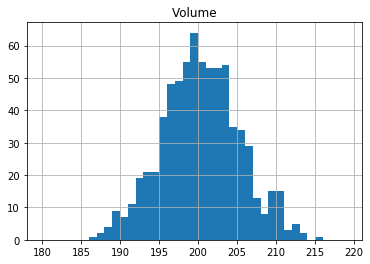
\includegraphics[width=0.6\textwidth]{figures/Untitled_40_1.png}
\end{figure}
%    { \hspace*{\fill} \\}

\begin{tcolorbox}[breakable, size=fbox, boxrule=1pt, pad at break*=1mm,colback=cellbackground, colframe=cellborder]
\begin{Verbatim}[commandchars=\\\{\}]
\PY{n}{df1}\PY{p}{[}\PY{l+s+s1}{\PYZsq{}}\PY{l+s+s1}{Volume}\PY{l+s+s1}{\PYZsq{}}\PY{p}{]} \PY{o}{=} \PY{p}{(}\PY{n}{df1}\PY{p}{[}\PY{l+s+s1}{\PYZsq{}}\PY{l+s+s1}{Volume}\PY{l+s+s1}{\PYZsq{}}\PY{p}{]} \PY{o}{\PYZhy{}} \PY{n}{df1}\PY{p}{[}\PY{l+s+s1}{\PYZsq{}}\PY{l+s+s1}{Volume}\PY{l+s+s1}{\PYZsq{}}\PY{p}{]}\PY{o}{.}\PY{n}{mean}\PY{p}{(}\PY{p}{)}\PY{p}{)} \PY{o}{/} \PY{n}{df1}\PY{p}{[}\PY{l+s+s1}{\PYZsq{}}\PY{l+s+s1}{Volume}\PY{l+s+s1}{\PYZsq{}}\PY{p}{]}\PY{o}{.}\PY{n}{std}\PY{p}{(}\PY{p}{)}

\PY{n}{df1}\PY{o}{.}\PY{n}{hist}\PY{p}{(}\PY{l+s+s1}{\PYZsq{}}\PY{l+s+s1}{Volume}\PY{l+s+s1}{\PYZsq{}}\PY{p}{,} \PY{n}{bins}\PY{o}{=}\PY{n}{np}\PY{o}{.}\PY{n}{arange}\PY{p}{(}\PY{o}{\PYZhy{}}\PY{l+m+mi}{5}\PY{p}{,} \PY{l+m+mi}{5}\PY{p}{,} \PY{l+m+mf}{0.1}\PY{p}{)}\PY{p}{)}
\PY{n+nb}{print} \PY{p}{(}\PY{n}{df1}\PY{p}{[}\PY{l+s+s1}{\PYZsq{}}\PY{l+s+s1}{Volume}\PY{l+s+s1}{\PYZsq{}}\PY{p}{]}\PY{o}{.}\PY{n}{mean}\PY{p}{(}\PY{p}{)}\PY{p}{)}
\PY{n+nb}{print} \PY{p}{(}\PY{n}{df1}\PY{p}{[}\PY{l+s+s1}{\PYZsq{}}\PY{l+s+s1}{Volume}\PY{l+s+s1}{\PYZsq{}}\PY{p}{]}\PY{o}{.}\PY{n}{std}\PY{p}{(}\PY{p}{)}\PY{p}{)}

-6.148550054609154e-15
1.0
\end{Verbatim}
\end{tcolorbox}

\begin{figure}[h]
\centering
  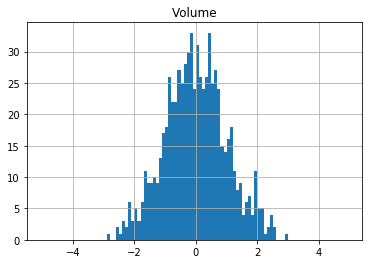
\includegraphics[width=0.6\textwidth]{figures/Untitled_41_1.png}
\end{figure}
  %  { \hspace*{\fill} \\}
    
\clearpage
\section{Plotting in \texttt{python}}\label{plotting-in-python}

As we have just seen \texttt{pandas} allows to quickly draw histograms of dataframe columns, but during an analysis we may want to plot distributions from \texttt{list} or objects not stored in a dataframe. Furthermore the simple and very useful provided interface doesn't grant full access to all histogram features that we need to produce nice and informative plots.

In order to do so we can use the \texttt{matplotlib} module which is specifically dedicated to plotting (pandas interface is based on the same module indeed). Let's look briefly to its capability by examples.

\subsection{Plot a graph given \(x\) and \(y\) values (scatter-plot)}\label{plot-a-graph-given-x-and-y-values}

\begin{tcolorbox}[breakable, size=fbox, boxrule=1pt, pad at break*=1mm,colback=cellbackground, colframe=cellborder]
\begin{Verbatim}[commandchars=\\\{\}]
\PY{k+kn}{from} \PY{n+nn}{matplotlib} \PY{k}{import} \PY{n}{pyplot} \PY{k}{as} \PY{n}{plt}

\PY{n}{x} \PY{o}{=} \PY{p}{[}\PY{l+m+mi}{1}\PY{p}{,} \PY{l+m+mi}{2}\PY{p}{,} \PY{l+m+mi}{3}\PY{p}{]}
\PY{n}{y} \PY{o}{=} \PY{p}{[}\PY{l+m+mf}{0.3}\PY{p}{,} \PY{l+m+mf}{0.4}\PY{p}{,} \PY{l+m+mf}{0.6}\PY{p}{]}
 
\PY{n}{plt}\PY{o}{.}\PY{n}{plot}\PY{p}{(}\PY{n}{x}\PY{p}{,} \PY{n}{y}\PY{p}{,} \PY{n}{marker}\PY{o}{=}\PY{l+s+s1}{\PYZsq{}}\PY{l+s+s1}{o}\PY{l+s+s1}{\PYZsq{}}\PY{p}{)} \PY{c+c1}{\PYZsh{} we are using circle markers}
\PY{n}{plt}\PY{o}{.}\PY{n}{grid}\PY{p}{(}\PY{k+kc}{True}\PY{p}{)}               \PY{c+c1}{\PYZsh{} this line activate grid drawing}
\PY{n}{plt}\PY{o}{.}\PY{n}{show}\PY{p}{(}\PY{p}{)}
\end{Verbatim}
\end{tcolorbox}

\begin{figure}[h]
\centering
  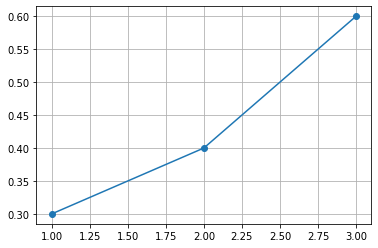
\includegraphics[width=0.6\textwidth]{figures/Untitled_43_0.png}
\end{figure}
%    { \hspace*{\fill} \\}
    
\begin{tcolorbox}[breakable, size=fbox, boxrule=1pt, pad at break*=1mm,colback=cellbackground, colframe=cellborder]
\begin{Verbatim}[commandchars=\\\{\}]
\PY{c+c1}{\PYZsh{} if we want to plot specific points too}

\PY{n}{x} \PY{o}{=} \PY{p}{[}\PY{l+m+mi}{1}\PY{p}{,} \PY{l+m+mi}{2}\PY{p}{,} \PY{l+m+mi}{3}\PY{p}{]}
\PY{n}{y} \PY{o}{=} \PY{p}{[}\PY{l+m+mf}{0.3}\PY{p}{,} \PY{l+m+mf}{0.4}\PY{p}{,} \PY{l+m+mf}{0.6}\PY{p}{]}
 
\PY{n}{plt}\PY{o}{.}\PY{n}{plot}\PY{p}{(}\PY{n}{x}\PY{p}{,} \PY{n}{y}\PY{p}{,} \PY{n}{marker}\PY{o}{=}\PY{l+s+s1}{\PYZsq{}}\PY{l+s+s1}{x}\PY{l+s+s1}{\PYZsq{}}\PY{p}{)}
\PY{n}{plt}\PY{o}{.}\PY{n}{plot}\PY{p}{(}\PY{l+m+mf}{2.5}\PY{p}{,} \PY{l+m+mf}{0.5}\PY{p}{,} \PY{n}{marker}\PY{o}{=}\PY{l+s+s1}{\PYZsq{}}\PY{l+s+s1}{X}\PY{l+s+s1}{\PYZsq{}}\PY{p}{,} \PY{n}{ms}\PY{o}{=}\PY{l+m+mi}{12}\PY{p}{,} \PY{n}{color}\PY{o}{=}\PY{l+s+s1}{\PYZsq{}}\PY{l+s+s1}{red}\PY{l+s+s1}{\PYZsq{}}\PY{p}{)}
\PY{n}{plt}\PY{o}{.}\PY{n}{plot}\PY{p}{(}\PY{l+m+mf}{1.5}\PY{p}{,} \PY{l+m+mf}{0.35}\PY{p}{,} \PY{n}{marker}\PY{o}{=}\PY{l+s+s1}{\PYZsq{}}\PY{l+s+s1}{x}\PY{l+s+s1}{\PYZsq{}}\PY{p}{,} \PY{n}{ms}\PY{o}{=}\PY{l+m+mi}{12}\PY{p}{,} \PY{n}{color}\PY{o}{=}\PY{l+s+s1}{\PYZsq{}}\PY{l+s+s1}{red}\PY{l+s+s1}{\PYZsq{}}\PY{p}{)}
\PY{n}{plt}\PY{o}{.}\PY{n}{grid}\PY{p}{(}\PY{k+kc}{True}\PY{p}{)}              
\PY{n}{plt}\PY{o}{.}\PY{n}{show}\PY{p}{(}\PY{p}{)}
\end{Verbatim}
\end{tcolorbox}

\begin{figure}[h]
\centering
  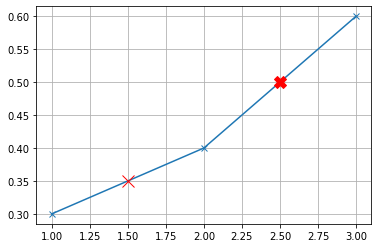
\includegraphics[width=0.6\textwidth]{figures/Untitled_44_0.png}
\end{figure}
%    { \hspace*{\fill} \\}
    
\subsubsection{What if \(x\) values are dates ?}

\begin{tcolorbox}[breakable, size=fbox, boxrule=1pt, pad at break*=1mm,colback=cellbackground, colframe=cellborder]
\begin{Verbatim}[commandchars=\\\{\}]
\PY{k+kn}{import} \PY{n+nn}{datetime}
\PY{k+kn}{import} \PY{n+nn}{matplotlib}\PY{n+nn}{.}\PY{n+nn}{dates} \PY{k}{as} \PY{n+nn}{mdates}

\PY{n}{x} \PY{o}{=} \PY{p}{[}\PY{n}{datetime}\PY{o}{.}\PY{n}{date}\PY{p}{(}\PY{l+m+mi}{2020}\PY{p}{,} \PY{l+m+mi}{7}\PY{p}{,} \PY{l+m+mi}{20}\PY{p}{)}\PY{p}{,}  \PY{n}{datetime}\PY{o}{.}\PY{n}{date}\PY{p}{(}\PY{l+m+mi}{2020}\PY{p}{,} \PY{l+m+mi}{7}\PY{p}{,} \PY{l+m+mi}{30}\PY{p}{)}\PY{p}{,} 
     \PY{n}{datetime}\PY{o}{.}\PY{n}{date}\PY{p}{(}\PY{l+m+mi}{2020}\PY{p}{,} \PY{l+m+mi}{8}\PY{p}{,} \PY{l+m+mi}{10}\PY{p}{)}\PY{p}{,}  \PY{n}{datetime}\PY{o}{.}\PY{n}{date}\PY{p}{(}\PY{l+m+mi}{2020}\PY{p}{,} \PY{l+m+mi}{8}\PY{p}{,} \PY{l+m+mi}{20}\PY{p}{)}\PY{p}{]}
     
\PY{n}{y} \PY{o}{=} \PY{p}{[}\PY{l+m+mi}{10}\PY{p}{,} \PY{l+m+mi}{20}\PY{p}{,} \PY{l+m+mi}{34}\PY{p}{,} \PY{l+m+mi}{45}\PY{p}{]}
\PY{n}{plt}\PY{o}{.}\PY{n}{plot}\PY{p}{(}\PY{n}{x}\PY{p}{,} \PY{n}{y}\PY{p}{,} \PY{n}{marker}\PY{o}{=}\PY{l+s+s1}{\PYZsq{}}\PY{l+s+s1}{o}\PY{l+s+s1}{\PYZsq{}}\PY{p}{)}
\PY{c+c1}{\PYZsh{} this line tells matplotlib we have dates on x axis}
\PY{n}{plt}\PY{o}{.}\PY{n}{gca}\PY{p}{(}\PY{p}{)}\PY{o}{.}\PY{n}{xaxis}\PY{o}{.}\PY{n}{set\PYZus{}major\PYZus{}formatter}\PY{p}{(}\PY{n}{mdates}\PY{o}{.}\PY{n}{DateFormatter}\PY{p}{(}\PY{l+s+s1}{\PYZsq{}}\PY{l+s+s1}{\PYZpc{}}\PY{l+s+s1}{Y\PYZhy{}}\PY{l+s+s1}{\PYZpc{}}\PY{l+s+s1}{m\PYZhy{}}\PY{l+s+si}{\PYZpc{}d}\PY{l+s+s1}{\PYZsq{}}\PY{p}{)}\PY{p}{)}
\PY{c+c1}{\PYZsh{} this one instead rotate labels to avoid superimposition}
\PY{n}{plt}\PY{o}{.}\PY{n}{xticks}\PY{p}{(}\PY{n}{rotation}\PY{o}{=}\PY{l+m+mi}{45}\PY{p}{)}
\PY{n}{plt}\PY{o}{.}\PY{n}{grid}\PY{p}{(}\PY{k+kc}{True}\PY{p}{)}
\PY{n}{plt}\PY{o}{.}\PY{n}{show}\PY{p}{(}\PY{p}{)}
\end{Verbatim}
\end{tcolorbox}

\begin{figure}[h]
\centering
  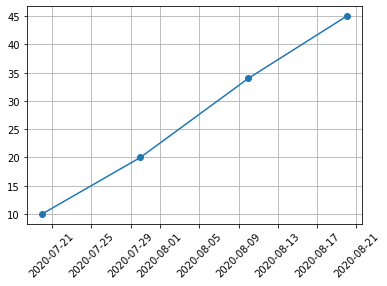
\includegraphics[width=0.6\textwidth]{figures/Untitled_46_0.png}
\end{figure}
%    { \hspace*{\fill} \\}
    
\subsection{Plotting an Histogram}\label{plotting-an-histogram}

\begin{tcolorbox}[breakable, size=fbox, boxrule=1pt, pad at break*=1mm,colback=cellbackground, colframe=cellborder]
\begin{Verbatim}[commandchars=\\\{\}]
\PY{k+kn}{import} \PY{n+nn}{random} 
\PY{n}{numbers} \PY{o}{=} \PY{p}{[}\PY{p}{]}
\PY{k}{for} \PY{n}{\PYZus{}} \PY{o+ow}{in} \PY{n+nb}{range}\PY{p}{(}\PY{l+m+mi}{1000}\PY{p}{)}\PY{p}{:}
  \PY{n}{numbers}\PY{o}{.}\PY{n}{append}\PY{p}{(}\PY{n}{random}\PY{o}{.}\PY{n}{randint}\PY{p}{(}\PY{l+m+mi}{1}\PY{p}{,} \PY{l+m+mi}{10}\PY{p}{)}\PY{p}{)}

\PY{k+kn}{from} \PY{n+nn}{matplotlib} \PY{k}{import} \PY{n}{pyplot} \PY{k}{as} \PY{n}{plt}

\PY{c+c1}{\PYZsh{} Here we define the binning}
\PY{c+c1}{\PYZsh{} 6 is the number of bins, going from 0 to 10}
\PY{n}{plt}\PY{o}{.}\PY{n}{hist}\PY{p}{(}\PY{n}{numbers}\PY{p}{,} \PY{l+m+mi}{10}\PY{p}{,} \PY{n+nb}{range}\PY{o}{=}\PY{p}{[}\PY{l+m+mi}{0}\PY{p}{,} \PY{l+m+mi}{11}\PY{p}{]}\PY{p}{)} 
\PY{n}{plt}\PY{o}{.}\PY{n}{show}\PY{p}{(}\PY{p}{)}
\end{Verbatim}
\end{tcolorbox}

\begin{figure}[h]
\centering
  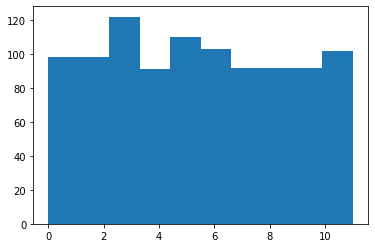
\includegraphics[width=0.55\textwidth]{figures/Untitled_48_0.png}
\end{figure}
 %   { \hspace*{\fill} \\}
    
\subsubsection{Plotting a Function}\label{plotting-a-function}

In this case let's try to make the plot prettier adding labels, legend\ldots{}
All the commands apply also to the previous examples.

\begin{tcolorbox}[breakable, size=fbox, boxrule=1pt, pad at break*=1mm,colback=cellbackground, colframe=cellborder]
\begin{Verbatim}[commandchars=\\\{\}]
\PY{k+kn}{import} \PY{n+nn}{numpy} \PY{k}{as} \PY{n+nn}{np}
\PY{k+kn}{import} \PY{n+nn}{matplotlib}\PY{n+nn}{.}\PY{n+nn}{pyplot} \PY{k}{as} \PY{n+nn}{plt}
\PY{k+kn}{from} \PY{n+nn}{scipy}\PY{n+nn}{.}\PY{n+nn}{stats} \PY{k}{import} \PY{n}{norm}

\PY{c+c1}{\PYZsh{} define the functions to plot}
\PY{c+c1}{\PYZsh{} a gaussian with mean=0  and sigma=1}
\PY{c+c1}{\PYZsh{} in scipy module this is called norm}
\PY{n}{mu}\PY{o}{=}\PY{l+m+mi}{0}
\PY{n}{sigma} \PY{o}{=} \PY{l+m+mi}{1}
\PY{n}{x} \PY{o}{=} \PY{n}{np}\PY{o}{.}\PY{n}{arange}\PY{p}{(}\PY{o}{\PYZhy{}}\PY{l+m+mi}{10}\PY{p}{,} \PY{o}{\PYZhy{}}\PY{l+m+mf}{1.645}\PY{p}{,} \PY{l+m+mf}{0.001}\PY{p}{)}
\PY{n}{x\PYZus{}all} \PY{o}{=} \PY{n}{np}\PY{o}{.}\PY{n}{arange}\PY{p}{(}\PY{o}{\PYZhy{}}\PY{l+m+mi}{4}\PY{p}{,} \PY{l+m+mi}{4}\PY{p}{,} \PY{l+m+mf}{0.001}\PY{p}{)}
\PY{n}{y} \PY{o}{=} \PY{n}{norm}\PY{o}{.}\PY{n}{pdf}\PY{p}{(}\PY{n}{x}\PY{p}{,} \PY{l+m+mi}{0}\PY{p}{,} \PY{l+m+mi}{1}\PY{p}{)}
\PY{n}{y\PYZus{}all} \PY{o}{=} \PY{n}{norm}\PY{o}{.}\PY{n}{pdf}\PY{p}{(}\PY{n}{x\PYZus{}all}\PY{p}{,} \PY{l+m+mi}{0}\PY{p}{,} \PY{l+m+mi}{1}\PY{p}{)}

\PY{c+c1}{\PYZsh{} draw the gaussian}
\PY{n}{plt}\PY{o}{.}\PY{n}{plot}\PY{p}{(}\PY{n}{x\PYZus{}all}\PY{p}{,} \PY{n}{y\PYZus{}all}\PY{p}{,} \PY{n}{label}\PY{o}{=}\PY{l+s+s1}{\PYZsq{}}\PY{l+s+s1}{Gaussian}\PY{l+s+s1}{\PYZsq{}}\PY{p}{)}

\PY{c+c1}{\PYZsh{} fill with different alpha using x\PYZus{}all and y\PYZus{}all as limits}
\PY{c+c1}{\PYZsh{} alpha set the transparency level: 0 trasparent, 1 solid}
\PY{n}{plt}\PY{o}{.}\PY{n}{fill\PYZus{}between}\PY{p}{(}\PY{n}{x\PYZus{}all}\PY{p}{,} \PY{n}{y\PYZus{}all}\PY{p}{,} \PY{l+m+mi}{0}\PY{p}{,} \PY{n}{alpha}\PY{o}{=}\PY{l+m+mf}{0.1}\PY{p}{,} \PY{n}{color}\PY{o}{=}\PY{l+s+s1}{\PYZsq{}}\PY{l+s+s1}{blue}\PY{l+s+s1}{\PYZsq{}}\PY{p}{,} \PY{n}{label}\PY{o}{=}\PY{l+s+s2}{\PYZdq{}}\PY{l+s+s2}{Gaussian CDF}\PY{l+s+s2}{\PYZdq{}}\PY{p}{)}

\PY{c+c1}{\PYZsh{} fill with color red using x and y as limits}
\PY{c+c1}{\PYZsh{} label associate text to the object for the legend}
\PY{n}{plt}\PY{o}{.}\PY{n}{fill\PYZus{}between}\PY{p}{(}\PY{n}{x}\PY{p}{,} \PY{n}{y}\PY{p}{,} \PY{l+m+mi}{0}\PY{p}{,} \PY{n}{alpha}\PY{o}{=}\PY{l+m+mi}{1}\PY{p}{,} \PY{n}{color}\PY{o}{=}\PY{l+s+s1}{\PYZsq{}}\PY{l+s+s1}{red}\PY{l+s+s1}{\PYZsq{}}\PY{p}{,} \PY{n}{label}\PY{o}{=}\PY{l+s+s2}{\PYZdq{}}\PY{l+s+s2}{5}\PY{l+s+s2}{\PYZpc{}}\PY{l+s+s2}{ tail}\PY{l+s+s2}{\PYZdq{}}\PY{p}{)}

\PY{c+c1}{\PYZsh{} set x axis limits}
\PY{n}{plt}\PY{o}{.}\PY{n}{xlim}\PY{p}{(}\PY{p}{[}\PY{o}{\PYZhy{}}\PY{l+m+mi}{4}\PY{p}{,} \PY{l+m+mi}{4}\PY{p}{]}\PY{p}{)}

\PY{c+c1}{\PYZsh{} add a label for X axis}
\PY{n}{plt}\PY{o}{.}\PY{n}{xlabel}\PY{p}{(}\PY{l+s+s2}{\PYZdq{}}\PY{l+s+s2}{Changes of value}\PY{l+s+s2}{\PYZdq{}}\PY{p}{)}

\PY{c+c1}{\PYZsh{} add a label to y axis}
\PY{n}{plt}\PY{o}{.}\PY{n}{ylabel}\PY{p}{(}\PY{l+s+s2}{\PYZdq{}}\PY{l+s+s2}{Gaussian values}\PY{l+s+s2}{\PYZdq{}}\PY{p}{)}

\PY{c+c1}{\PYZsh{} add histogram title}
\PY{n}{plt}\PY{o}{.}\PY{n}{title}\PY{p}{(}\PY{l+s+s2}{\PYZdq{}}\PY{l+s+s2}{Distribution of changes of value}\PY{l+s+s2}{\PYZdq{}}\PY{p}{)}

\PY{c+c1}{\PYZsh{} draw a vertical line at x=\PYZhy{}1.645}
\PY{c+c1}{\PYZsh{} y limits are in percent w.r.t. to y axis length}
\PY{n}{plt}\PY{o}{.}\PY{n}{axvline}\PY{p}{(}\PY{n}{x}\PY{o}{=}\PY{o}{\PYZhy{}}\PY{l+m+mf}{1.645}\PY{p}{,} \PY{n}{ymin}\PY{o}{=}\PY{l+m+mf}{0.1}\PY{p}{,} \PY{n}{ymax}\PY{o}{=}\PY{l+m+mi}{1}\PY{p}{,} \PY{n}{linestyle}\PY{o}{=}\PY{l+s+s1}{\PYZsq{}}\PY{l+s+s1}{:}\PY{l+s+s1}{\PYZsq{}}\PY{p}{,} \PY{n}{linewidth}\PY{o}{=}\PY{l+m+mi}{1}\PY{p}{,} \PY{n}{color} \PY{o}{=} \PY{l+s+s1}{\PYZsq{}}\PY{l+s+s1}{red}\PY{l+s+s1}{\PYZsq{}}\PY{p}{)}

\PY{c+c1}{\PYZsh{} write some text to explain the line}
\PY{n}{plt}\PY{o}{.}\PY{n}{text}\PY{p}{(}\PY{o}{\PYZhy{}}\PY{l+m+mf}{1.9}\PY{p}{,} \PY{o}{.}\PY{l+m+mi}{12}\PY{p}{,} \PY{l+s+s1}{\PYZsq{}}\PY{l+s+s1}{95}\PY{l+s+s1}{\PYZpc{}}\PY{l+s+s1}{ percentile (VaR loss)}\PY{l+s+s1}{\PYZsq{}}\PY{p}{,}\PY{n}{fontsize}\PY{o}{=}\PY{l+m+mi}{10}\PY{p}{,} \PY{n}{rotation}\PY{o}{=}\PY{l+m+mi}{90}\PY{p}{,} 
                                    \PY{n}{color}\PY{o}{=}\PY{l+s+s1}{\PYZsq{}}\PY{l+s+s1}{red}\PY{l+s+s1}{\PYZsq{}}\PY{p}{)}

\PY{n}{plt}\PY{o}{.}\PY{n}{legend}\PY{p}{(}\PY{p}{)}
\PY{n}{plt}\PY{o}{.}\PY{n}{show}\PY{p}{(}\PY{p}{)}
\end{Verbatim}
\end{tcolorbox}

\begin{figure}[htp]
\centering
  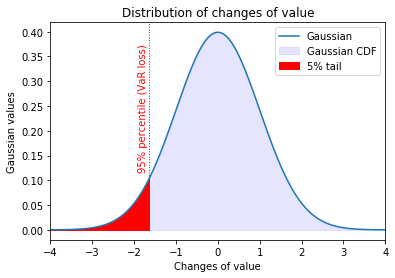
\includegraphics[width=0.55\textwidth]{figures/Untitled_50_0.png}
\end{figure}
%    { \hspace*{\fill} \\}
    \clearpage
If you are particularly satisfied by your work you can save the graph to a file:

\begin{tcolorbox}[breakable, size=fbox, boxrule=1pt, pad at break*=1mm,colback=cellbackground, colframe=cellborder]
\begin{Verbatim}[commandchars=\\\{\}]
\PY{n}{plt}\PY{o}{.}\PY{n}{savefig}\PY{p}{(}\PY{l+s+s1}{\PYZsq{}}\PY{l+s+s1}{normal\PYZus{}curve.png}\PY{l+s+s1}{\PYZsq{}}\PY{p}{)}

<Figure size 432x288 with 0 Axes>

\end{Verbatim}
\end{tcolorbox}
